The aim of this task is to compute a desired input state curve and create an optimal trajectory that minimizes the cost with respect to this desired curve. 

\section{Equilibrium computation}
The desired curve is required to start and end in equilibrium points for the system. We don't consider the trivial equilibrium for a set position, namely 
\begin{align*}
 f_1(x_t,u_t)=0 \\
 f_2(x_t,u_t)=0 \\
 f_3(x_t,u_t)=0 \\
\end{align*}
Which implies $x_4=x_5=x_6=0$, as they wouldn't give us an insightful understanding of the system behavior.
We instead considered the so called cornering equilibria of the system, for which the following holds:
\begin{align*}
 f_1(x_t,u_t) \neq 0 \\
 f_2(x_t,u_t) \neq 0 \\
 f_3(x_t,u_t) \neq 0 \\
 f_4(x_t,u_t)=0 \\
 f_5(x_t,u_t)=0 \\
 f_6(x_t,u_t)=0 
\end{align*}
This trajectories can be characterized as either a uniform linear or a uniform circular movement. 
Since the states $x_1, x_2, x_3$ do not have a role in the dynamics for the last three states, as they are just integrated from the latter, we can find these cornering equilibria by studying the reduced system

\begin{align*}
	m \dot{x_4} = F_{y,r} \sin x_5 + u_2 \cos (x_5 - u_1) + F_{y,f} \sin (x_5 - u_1) \\
    \dot{x_5} = \frac{1} {m x_4} (F_{y,r} \cos x_5 + F_{y,f} \cos(x_5 - u_1) - u_2 \sin (x_5 - u_1))-x_6
    \\
    I_z \dot{x_6} = (u_1 \sin u_1 + F_{y,f}\cos u_1 )a - F_{y,r} b   
\end{align*}
 
Which is a three equation system in five variables. This means we have two degrees of freedom in choosing the desired equilibrium variables, and find the others by solving the system. 
We decided to set the velocity module $x_4$ and the velocity angle $x_5$. We've found the other equilibrium values for the system with a zero finding method, using \texttt{sp.fsolve} from the scipy toolbox. \\
By imposing $(x_4^1, x_5^1)=(8, 0)$ and $(x_4^1, x_5^1)=(12, \frac{\pi}{6})$ we have found the cornering equilibrium pairs for the system dynamics.
\\ We proceeded by integrating the dynamics, which is useful both to check the values and to create the desired curve. The complete desired curve is computed by concatenating the two subtrajectories. 
\begin{figure}[!h]
	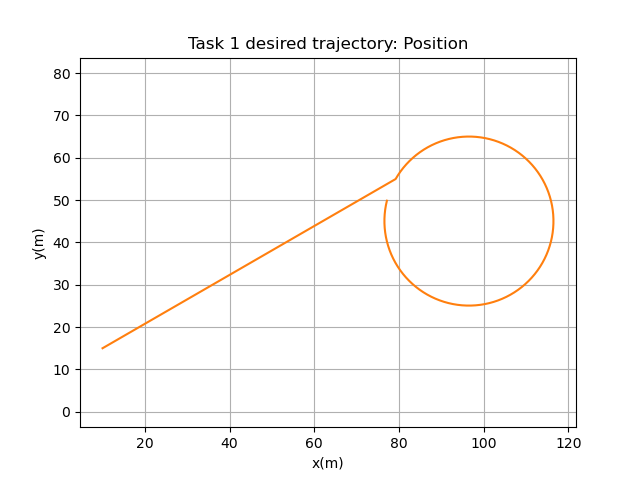
\includegraphics[width=\linewidth]{figs/destraj.png}
	\caption{Desired step position trajectory}
\end{figure} 

\begin{figure}[!h]
	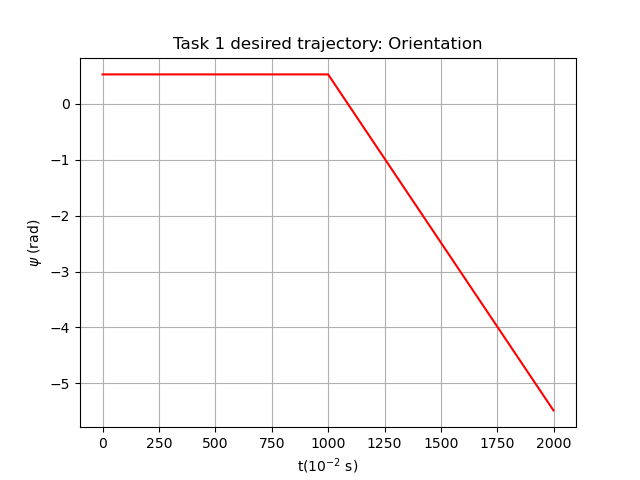
\includegraphics[width=\linewidth]{figs/despsi.png}
	\caption{Desired step $\psi$ trajectory}

	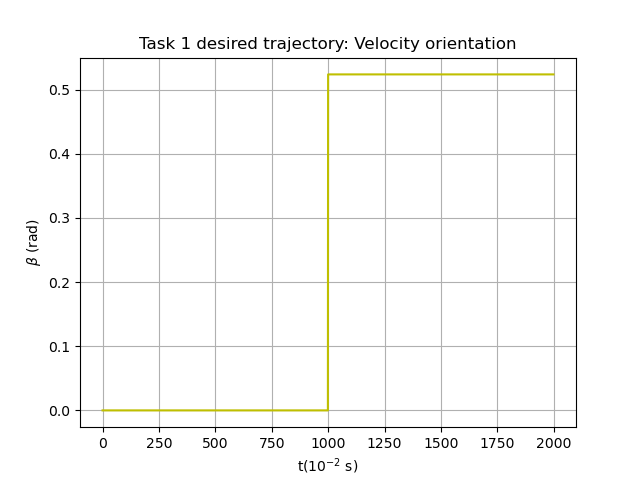
\includegraphics[width=\linewidth]{figs/desbeta.png}
	\caption{Desired step $\beta$ trajectory}
\end{figure} 

\begin{figure}[!h]
	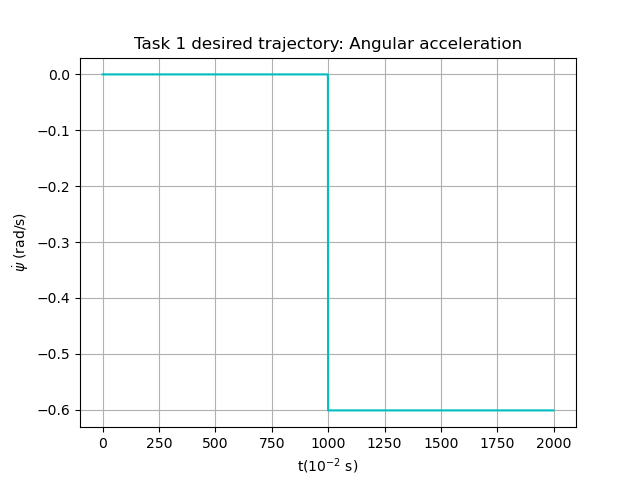
\includegraphics[width=\linewidth]{figs/despsid.png}
	\caption{Desired step $\dot{\psi}$ trajectory}
\end{figure} 

\FloatBarrier
\section{Optimal trajectory via Newton's algorithm}
To find an optimal trajectory between the two equilibria we will use a cost function that involves
the concept of quadratic form that allows us to input as parameters two weight matrices that represents how much
we want to track accurately a variable. The first weight matrix \texttt{QQt = 0.01*diag(0.1, 0.1, 100, 10, 100, 100)} 
is used for the state variables while the second one \texttt{RRt = 0.01*diag(5000, 0.00001)} is for the input variables.
\\This cost function will be minimized via a Newton's method, for the computation of the descent direction,
in which we can avoid to compute the Hessian of the dynamics by solving the costate equations and solving an affine linear quadratic problem;
and with a step size ($\gamma$) chosen by the Armijo's rule.
\\Additionally by using the shooting method we can further simplify the problem and consider it as unconstrained optimization problem with a 
single decision variable $u$.
\\To sum up the decision variable $u$ will be updated as:
\begin{align*}
	u_t^{k+1}=u_t^k+\gamma^k\Delta u_t^k\\
	x_t^{k+1}=f_t(x_t^{k+1},u_t^{k+1})
\end{align*}
The plots for which we need to pay more attention are the Armijo's one, in fact is possible to see if the algorithm is properly working,
if we are moving in the correct direction and if the step size chosen is the correct one or is outside of the admissible area between
the green and red lines. The following plots are taken every two iteration of the code.
\begin{figure}[!b]
	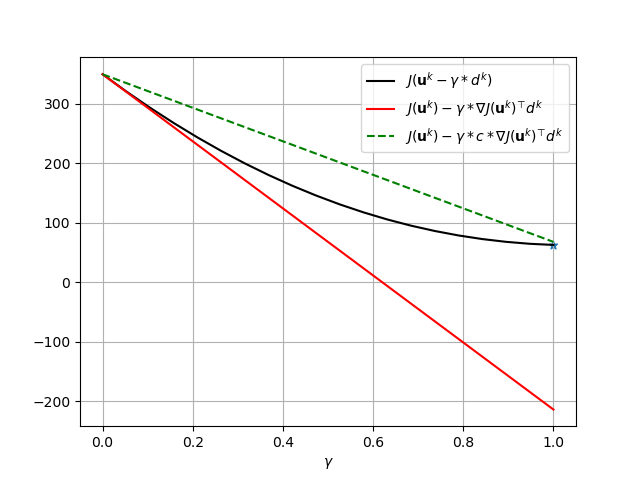
\includegraphics[width=0.5\columnwidth]{figs/Arm0.png}
	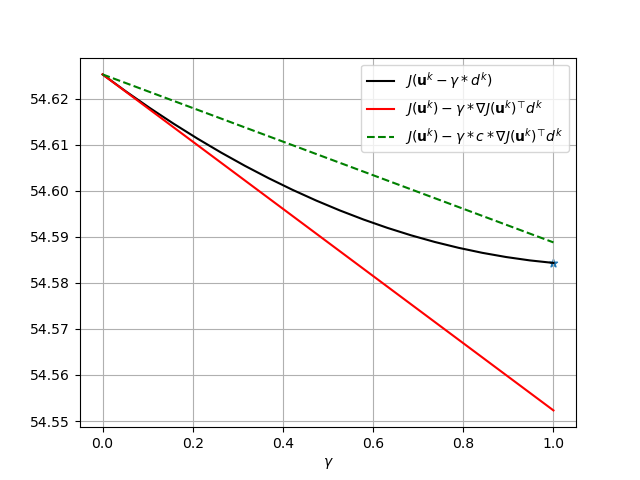
\includegraphics[width=0.5\columnwidth]{figs/arm2.png}
	\caption{Armijo's plot at the first and third iteration}
\end{figure}
\begin{figure}[ht]
	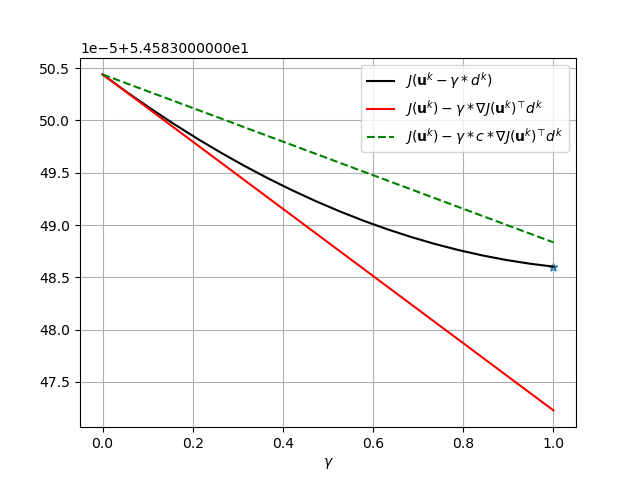
\includegraphics[width=0.5\linewidth]{figs/arm4.png}
    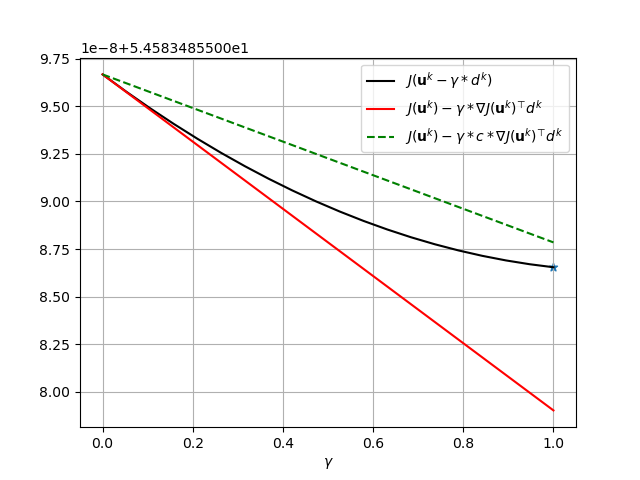
\includegraphics[width=0.5\linewidth]{figs/arm6.png}
	\caption{Armijo's plot at the fifth and seventh iteration}    
\end{figure} 

\begin{figure}[ht]
	\center
	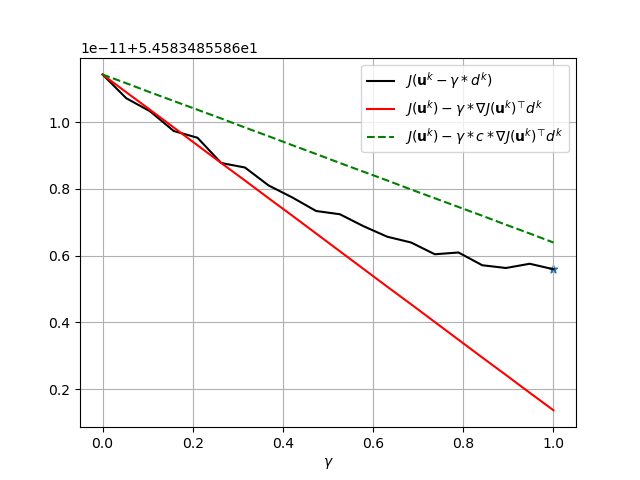
\includegraphics[width=0.75\linewidth]{figs/arm8.png}
	\caption{Armijo's plot at the last iteration}
	\label{fig:lastArm}
\end{figure} 

\FloatBarrier
As we can see from figure \ref{fig:lastArm} the algorithm is getting very close to the chosen sample period of the discretization and the result 
is that the curves are no longer so exact as in the first iterations so the central curve is no longer tangent to the red line.\\
In the following we can se the result of the applied methods on the obtained trajectories of the states and the inputs applied to the system.
\begin{figure}[htp]
    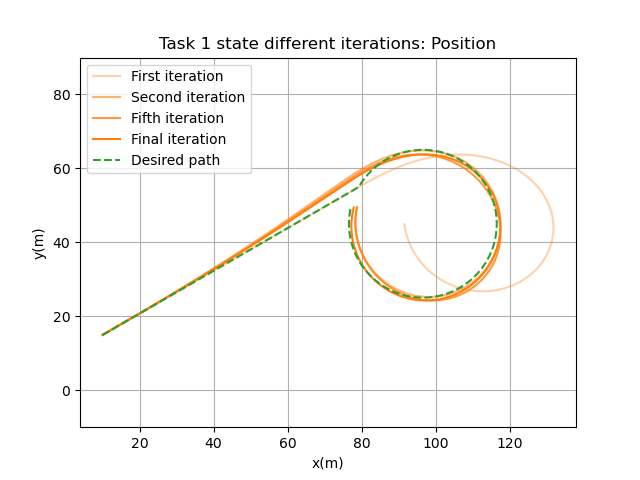
\includegraphics[width=0.5\textwidth]{figs/sometraj.png}
    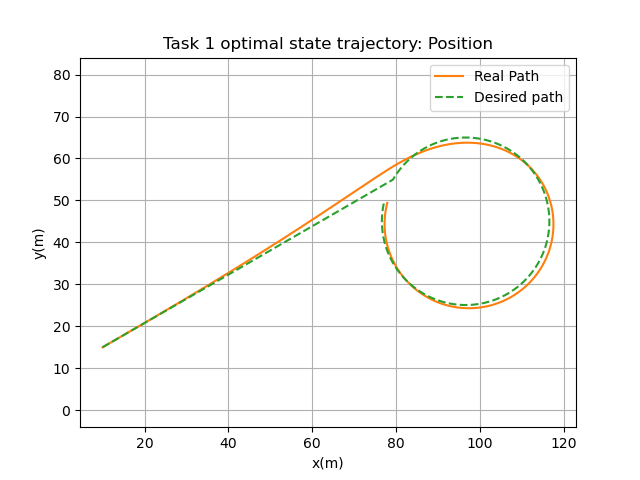
\includegraphics[width=0.5\textwidth]{figs/onetraj.png}
    \caption{Desired and obtained step position trajectory}
\end{figure}

\begin{figure}[htp]
    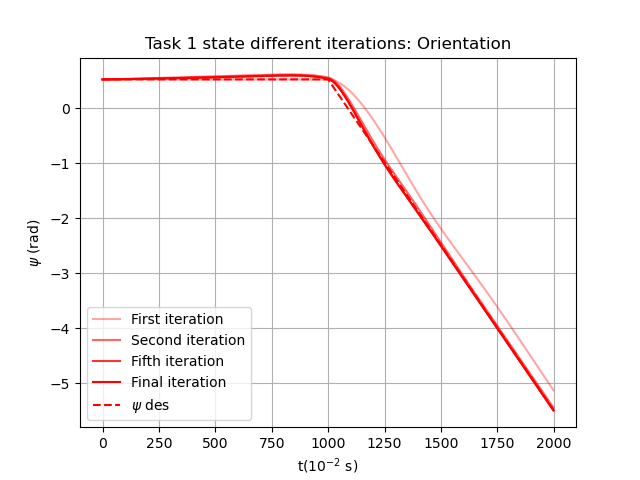
\includegraphics[width=0.5\textwidth]{figs/someorient.png}
    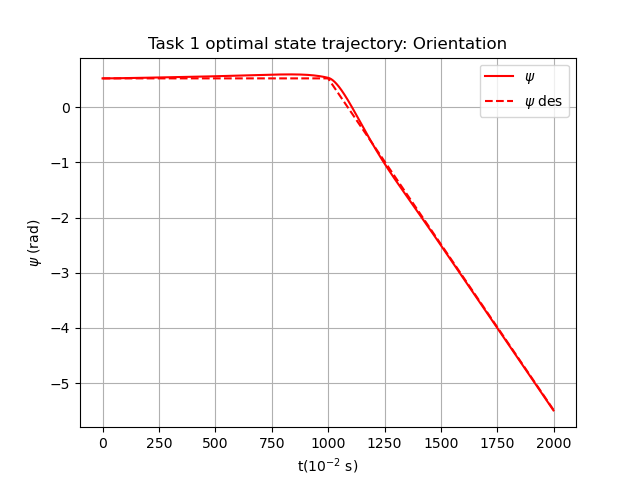
\includegraphics[width=0.5\textwidth]{figs/onepsi.png}
    \caption{Desired and obtained step orientation ($\psi$) trajectory}
\end{figure}

\begin{figure}[htp]
    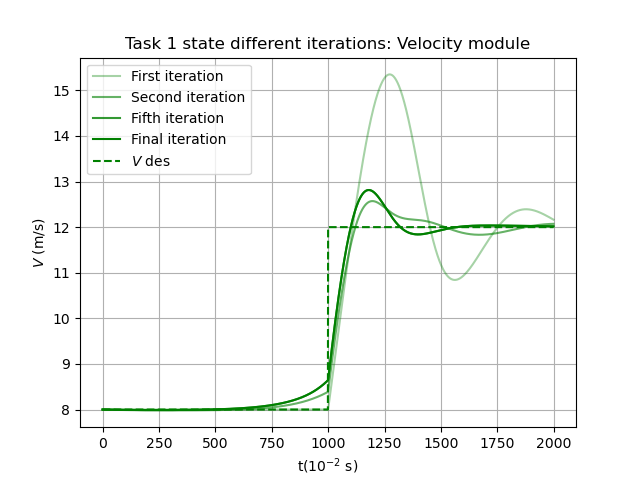
\includegraphics[width=0.5\textwidth]{figs/someV.png}
    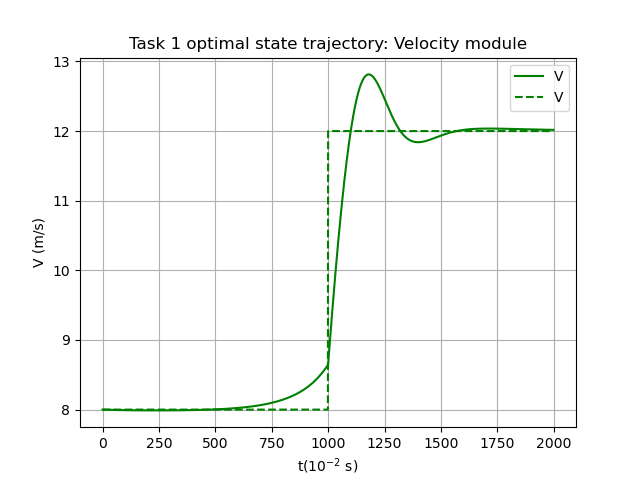
\includegraphics[width=0.5\textwidth]{figs/oneV.png}
    \caption{Desired and obtained step velocity trajectory}
\end{figure}

\begin{figure}[htp]
    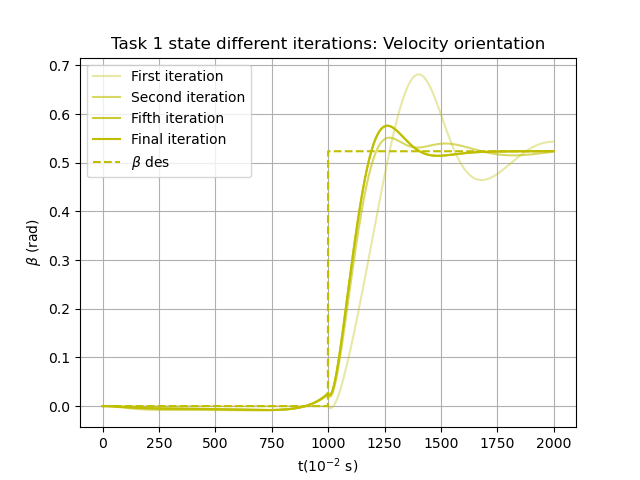
\includegraphics[width=0.5\textwidth]{figs/somebeta.png}
    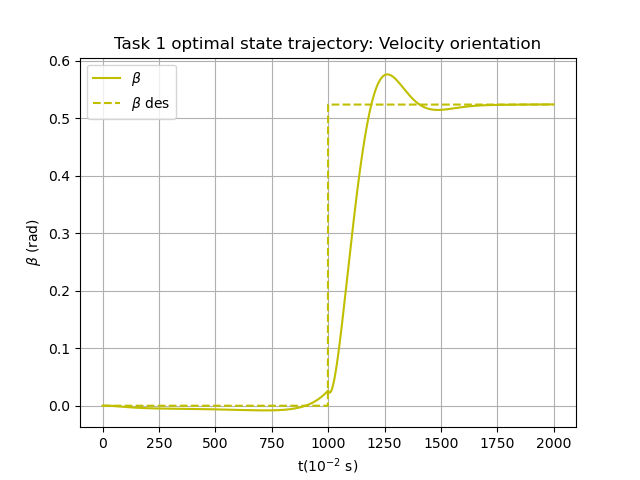
\includegraphics[width=0.5\textwidth]{figs/onebeta.png}
    \caption{Desired and obtained step $\beta$ trajectory}
\end{figure}

\begin{figure}[htp]
    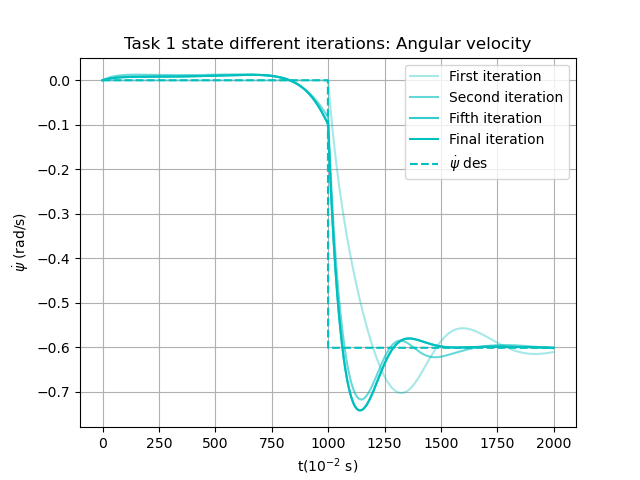
\includegraphics[width=0.5\textwidth]{figs/somepsid.png}
    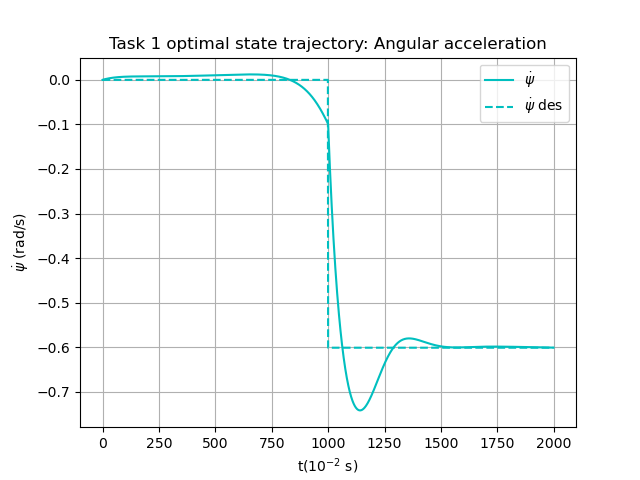
\includegraphics[width=0.5\textwidth]{figs/onepsid.png}
    \caption{Desired and obtained step $\dot{\psi}$ trajectory}
\end{figure}

\begin{figure}[htp]
    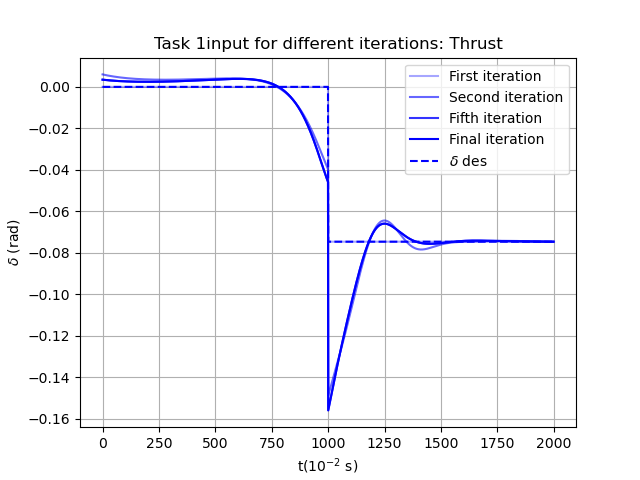
\includegraphics[width=0.5\textwidth]{figs/somedelta.png}
    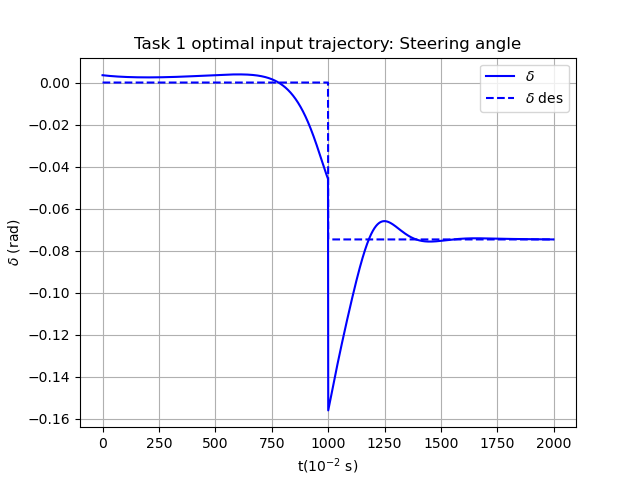
\includegraphics[width=0.5\textwidth]{figs/onedelta.png}
    \caption{Desired and obtained step $\delta$ trajectory}
	\label{fig:dstep}
\end{figure}

\begin{figure}[htp]
    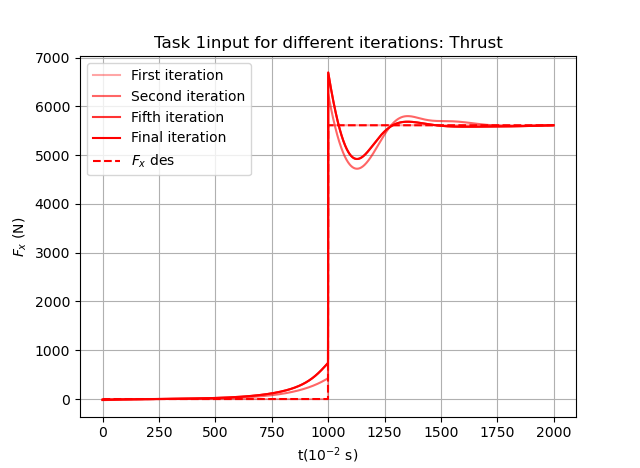
\includegraphics[width=0.5\textwidth]{figs/somefx.png}
    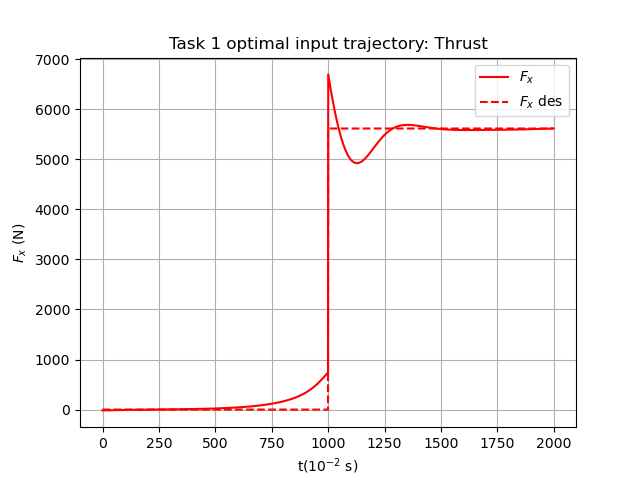
\includegraphics[width=0.5\textwidth]{figs/onefx.png}
    \caption{Desired and obtained step $F_x$ trajectory}
	\label{fig:fstep}
\end{figure}

\begin{figure}[htp]
    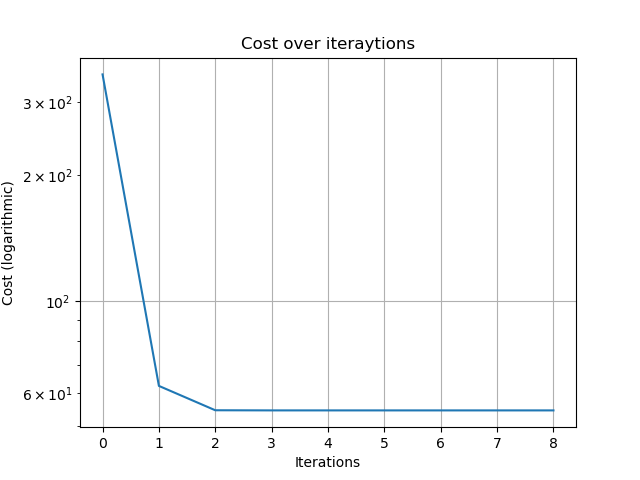
\includegraphics[width=0.5\textwidth]{figs/cost.png}
    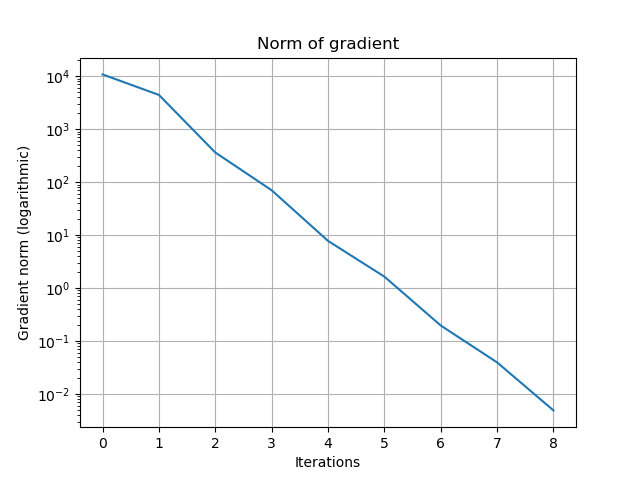
\includegraphics[width=0.5\textwidth]{figs/norm.png}
    \caption{Obtained decrease in cost function and norm of descent direction}
\end{figure}

\FloatBarrier
\section{Conclusions}
As we can see from figures \ref{fig:dstep} and \ref{fig:fstep} the request of a step change between the two equilibria
causes some overshoot in the control inputs in particular in $\delta$, however both the control inputs then stabilize at the desired values.
We found the values of the input cost matrix \texttt{RRt} to be extremely relevant: since the force $F_x$ is five orders of
magnitude greater than the other values, we had to take a very small penalty to that term in order to balance it.\\
We assumed this is due to the fact that the Newton's method uses a second order approximation and this outlier input value
could make the higher order terms more relevant in the computations.  